\documentclass[10pt,journal,comsoc]{IEEEtran}
% \documentclass[10pt,peerreview,comsoc]{IEEEtran}
% \documentclass[10pt,peerreviewca,comsoc]{IEEEtran}

\usepackage{amsmath,amsfonts}
\usepackage{amsthm}
\usepackage{array}
% \usepackage{algorithmic}
% \usepackage[caption=false,font=normalsize,labelfont=sf,textfont=sf]{subfig}
\usepackage{textcomp}
\usepackage{stfloats}
\usepackage{url}
\usepackage{verbatim}
\usepackage{graphicx}
\usepackage{cite}
\hyphenation{op-tical net-works semi-conduc-tor IEEE-Xplore}
% updated with editorial comments 8/9/2021



%%%% User defined
\usepackage{amssymb}
\usepackage{color,xcolor}

\usepackage{algorithm}
\usepackage{algpseudocode}
%
\usepackage[nice]{nicefrac}
\usepackage{orcidlink}    
\usepackage{bm,bbm,mathtools}
% \usepackage{caption}
\usepackage{subcaption}
% \usepackage{wrapfig}
% \usepackage{breqn}
\usepackage{multirow}
%
\def\P{{\mathbb P}} 
\def\p{{p}}
\def\Q{{\bm Q}} 
\def\E{{\mathbb E}} 
\DeclareMathOperator*{\argmax}{arg\,max}
\DeclareMathOperator*{\argmin}{arg\,min}
\newcommand*\dif{\,\mathrm{d}}
\newcommand\numberthis{\addtocounter{equation}{1}\tag{\theequation}}
\newtheorem{lemma}{Lemma}
\newtheorem{proposition}{Proposition}
\newtheorem{corollary}{Corollary}
\newtheorem{theorem}{Theorem}
\newcommand{\qmax}{Q_{\mathrm{max}}}
\newcommand{\nrb}{N_{\mathrm{RB}}}
\newcommand{\nre}{N_{\mathrm{RE}}}\newcommand{\dserv}{D_{\mathrm{s}}}
\newcommand{\dwait}{D_{\mathrm{w}}}
\newcommand{\dwaitCap}{\hat{D}_{\mathrm{w}}}
\newcommand{\dtot}{D}
\newcommand{\dvp}{\mathcal{D}}
\newcommand{\snr}{\gamma}
\newcommand{\snrInst}{{S}}
\newcommand{\hvar}{{\mu_{h^2}}}
\newcommand{\ddecod}{{\zeta}}
\definecolor{iG}{rgb}{0.0, 0.7, 0.0}
\def\OJlogo{\vspace{-4pt}\includegraphics[height=18pt]{Figures/new_logo.eps}}
\def\seclogo{\vspace{10pt}\includegraphics[height=18pt]{Figures/new_logo.eps}}
\def\authorrefmark#1{\ensuremath{^{\textbf{#1}}}}

\begin{document}
\title{Delay Analysis of 5G HARQ in the Presence of Decoding and Feedback Latencies}
\author{Vishnu N Moothedath\orcidlink{0000-0002-2739-5060}, 
        Sangwon Seo\orcidlink{0000-0002-9181-9454},
        Neda Petreska\orcidlink{0000-0002-2743-5800},
        Bernhard Kloiber,
        James Gross\orcidlink{0000-0001-6682-6559} 
        % <-this % stops a space
\thanks{This work has been submitted to the IEEE for possible publication.  Copyright may be transferred without notice, after which this version may no longer be accessible.}
\thanks{Vishnu N Moothedath, Sangwon Seo, and James Gross are with the Department of Intelligent Systems, KTH Royal Institute of Technology, Stockholm, Sweden (e-mail: vnmo@kth.se, sangwon@kth.se, jamesgr@kth.se).}% <-this % stops a space
\thanks{Neda Petreska and Bernhard Kloiber are with Siemens AG, Munich, Germany (e-mail: neda.petreska@siemens.com, bernhard.kloiber@siemens.com).}% <-this % stops a space
% \thanks{Thanks: We appreciate the valuable inputs from our colleague, Sahar Imtiaz.}
}

% \author{%Vishnu, Sangwon, James et.al.
%           Vishnu N Moothedath\orcidlink{0000-0002-2739-5060}$^{\dagger}$,
%            Sangwon Seo\orcidlink{0000-0002-9181-9454}$^{\dagger}$,
%            Neda Petreska\orcidlink{0000-0002-2743-5800}$^{\mathsection}$,
%            Bernhard Kloiber$^{\mathsection}$,
%            James Gross\orcidlink{0000-0001-6682-6559}$^{\dagger}$\\%
%           % <-this % stops a space
%           $^{\dagger}$\{vnmo, sangwon, jamesgr\}@kth.se, $^{\mathsection}$\{neda.petreska, bernhard.kloiber\}@siemens.com\\
%           % \{vnmo, sangwon, jamesgr\}@kth.se\\
%           % <-this % stops a space
%           $^{\dagger}$Department of Intelligent Systems, KTH Royal Institute of Technology, Stockholm, Sweden\\
%           $^{\mathsection}$Siemens AG, Munich, Germany
%           % <-this % stops a space
% % \thanks{Acknowledgement}% <-this % stops a space
% % \thanks{Thanks: We appreciate the valuable inputs from our colleague, Sahar Imtiaz.}
% }


%%%%%%%%%%%%%%%%%%%%%%%%%%%%%%%%%%%% 
% The paper headers
% \markboth{Journal of \LaTeX\ Class Files,~Vol.~14, No.~8, August~2021}%
% {Shell \MakeLowercase{\textit{et al.}}: A Sample Article Using IEEEtran.cls for IEEE Journals}

% \IEEEpubid{0000--0000/00\$00.00~\copyright~2021 IEEE}
% Remember, if you use this you must call \IEEEpubidadjcol in the second
% column for its text to clear the IEEEpubid mark.
%%%%%%%%%%%%%%%%%%%%%%%%%%%%%%%%%%%%

\maketitle
\begin{abstract}
The growing demand for stringent quality of service (QoS) guarantees in 5G networks requires accurate characterisation of delay performance, often measured using Delay Violation Probability (DVP) for a given target delay. Widely used retransmission schemes like Automatic Repeat reQuest (ARQ) and Hybrid ARQ (HARQ) improve QoS through effective feedback, incremental redundancy (IR), and parallel retransmission processes. However, existing works to quantify the DVP under these retransmission schemes overlook practical aspects such as decoding complexity, feedback delays, and the resulting need for multiple parallel ARQ/HARQ processes that enable packet transmissions without waiting for previous feedback, thus exploiting valuable transmission opportunities. This work proposes a comprehensive multi-server delay model for ARQ/HARQ that incorporates these aspects. Using a finite blocklength error model, we derive closed-form expressions and algorithms for accurate DVP evaluation under realistic 5G configurations aligned with 3GPP standards. Our numerical evaluations demonstrate notable improvements in DVP accuracy over the state-of-the-art, highlight the impact of parameter tuning and resource allocation, and reveal how DVP affects system throughput. 
\end{abstract}

\begin{IEEEkeywords}
5G, HARQ, QoS, delay violation probability (DVP), decoding complexity.
\end{IEEEkeywords}

% \tableofcontents
\IEEEpeerreviewmaketitle
% \clearpage

\section{Introduction}\label{sec:Intro} 


Novel view synthesis offers a fundamental approach to visualizing complex scenes by generating new perspectives from existing imagery. 
This has many potential applications, including virtual reality, movie production and architectural visualization \cite{Tewari2022NeuRendSTAR}. 
An emerging alternative to the common RGB sensors are event cameras, which are  
 bio-inspired visual sensors recording events, i.e.~asynchronous per-pixel signals of changes in brightness or color intensity. 

Event streams have very high temporal resolution and are inherently sparse, as they only happen when changes in the scene are observed. 
Due to their working principle, event cameras bring several advantages, especially in challenging cases: they excel at handling high-speed motions 
and have a substantially higher dynamic range of the supported signal measurements than conventional RGB cameras. 
Moreover, they have lower power consumption and require varied storage volumes for captured data that are often smaller than those required for synchronous RGB cameras \cite{Millerdurai_3DV2024, Gallego2022}. 

The ability to handle high-speed motions is crucial in static scenes as well,  particularly with handheld moving cameras, as it helps avoid the common problem of motion blur. It is, therefore, not surprising that event-based novel view synthesis has gained attention, although color values are not directly observed.
Notably, because of the substantial difference between the formats, RGB- and event-based approaches require fundamentally different design choices. %

The first solutions to event-based novel view synthesis introduced in the literature demonstrate promising results \cite{eventnerf, enerf} and outperform non-event-based alternatives for novel view synthesis in many challenging scenarios. 
Among them, EventNeRF \cite{eventnerf} enables novel-view synthesis in the RGB space by assuming events associated with three color channels as inputs. 
Due to its NeRF-based architecture \cite{nerf}, it can handle single objects with complete observations from roughly equal distances to the camera. 
It furthermore has limitations in training and rendering speed: 
the MLP used to represent the scene requires long training time and can only handle very limited scene extents or otherwise rendering quality will deteriorate. 
Hence, the quality of synthesized novel views will degrade for larger scenes. %

We present Event-3DGS (E-3DGS), i.e.,~a new method for novel-view synthesis from event streams using 3D Gaussians~\cite{3dgs} 
demonstrating fast reconstruction and rendering as well as handling of unbounded scenes. 
The technical contributions of this paper are as follows: 
\begin{itemize}
\item With E-3DGS, we introduce the first approach for novel view synthesis from a color event camera that combines 3D Gaussians with event-based supervision. 
\item We present frustum-based initialization, adaptive event windows, isotropic 3D Gaussian regularization and 3D camera pose refinement, and demonstrate that high-quality results can be obtained. %

\item Finally, we introduce new synthetic and real event datasets for large scenes to the community to study novel view synthesis in this new problem setting. 
\end{itemize}
Our experiments demonstrate systematically superior results compared to EventNeRF \cite{eventnerf} and other baselines. 
The source code and dataset of E-3DGS are released\footnote{\url{https://4dqv.mpi-inf.mpg.de/E3DGS/}}. 





\section{System Model and Problem Statement}\label{sec:model}
\begin{figure*}[th]
\centering
\begin{minipage}[t]{.5\textwidth}
  \centering
  \includegraphics[width=\textwidth]{Figures/model.eps}
  \caption{Illustration of the closed-loop communication system studied showing the retransmission process. Different delay components are shown where the packets experience them.}
  \label{fig:BasicModel}
\end{minipage}%
\hspace{0.03\textwidth}%
\begin{minipage}[t]{0.46\textwidth}
  \centering
  \includegraphics[width=\textwidth]{Figures/timingDiagram1.eps}
  \caption{Timing diagram showing the order and positions of different slot-based arrival and departure events with respect to the corresponding slot boundary.}
  \label{fig:timingdiagram}
\end{minipage}
\end{figure*}


Consider a 5G communication system as depicted in Fig.~\ref{fig:BasicModel}. 
A User Equipment (UE) generates or receives uplink (UL) packets and queues them for transmission\footnote{The analysis and results apply to uplink and downlink scenarios; we focus on the uplink for clarity and consistency.}. 
These packets are sent to a dedicated gNB via a 5G-NR wireless link, utilizing a fixed number of resources scheduled to the UE in each time slot.
The packet is encoded over these pre-allocated frequency domain resource blocks (RB) using the configured modulation and coding scheme (MCS).

If the queue is non-empty, the UE uses the entire slot to transmit the head-of-the-queue packet. 
The gNB attempts to decode the packet using the implemented coding scheme. Successful packets are used for their intended purpose, and an acknowledgement is fed back in the downlink (DL)
The UE receives this feedback, and retransmission is triggered if necessary. 
For this, a static retransmission scheme is configured, and the packets are discarded after a maximum number of transmission attempts.

The process involves various delays, as shown in Fig.~\ref{fig:BasicModel}. 
Encoding delay is ignored, as it occurs only once per packet and can be performed while the packet waits in the queue. Similarly, propagation delays are neglected due to the short distances typical in high-reliability applications. 
However, if needed, one can include the encoding delay by subtracting it from the delay target, as it is endured only once per packet, and the propagation delay by adding it to the decoding delay, as they are always encountered as a pair.



% \begin{figure*}[th]
% \centering
% \begin{minipage}{.48\textwidth}
%   \centering
%   \includegraphics[width=\textwidth]{Figures/model.eps}
%   \caption{Illustration showing the communication process. The different delay components are shown.}
%   \label{fig:BasicModel}
% \end{minipage}%
% \hspace{0.01\textwidth}%
% \begin{minipage}{0.33\textwidth}
%   \centering
%   \includegraphics[width=\textwidth]{Figures/timingDiagram.png}
%   \caption{Timing diagram showing the positions and order of different arrival and departure events.}
%   \label{fig:timingdiagram}
% \end{minipage}%
% \hspace{0.01\textwidth}%
% \begin{minipage}{0.16\textwidth}
%   \centering
%   \includegraphics[width=\textwidth]{Figures/harq.png}
%   \caption{Illustration of the HARQ-IR process with 4 redundancy versions.}
%   \label{fig:harqprocess}
% \end{minipage}
% \end{figure*}


\subsection{System Model}
Arrivals (or generation) of packets of size $n$ bits are modelled to occur randomly with an arrival probability of $f$.
While earlier arriving packets are given initial transmission opportunities, they do not wait for the feedback of previously transmitted packets, forming multiple simultaneous transmit-retransmit processes.
These packets form a queue awaiting transmission opportunities, which is modelled as a multi-server queue, with each server representing a packet undergoing a transmission process.
The maximum queue size is $\qmax$, and the slot length is $T$. 


New or retransmitted packets are added to the queue at the UE immediately after the slot boundary. 
Each packet transmission uses all time domain resources within the slot, with departures or feedback generation occurring at the gNB just before the subsequent slot boundary, as illustrated in Fig.~\ref{fig:timingdiagram}. Although the slot timings at the UE and gNB may not align perfectly in terms of absolute clock time due to propagation delay, their offset remains constant. Synchronization of slot indices is maintained through the application of a timing advance (TA) computed during the initial handshake, ensuring that a transmission in slot $k$ of the UE is received within slot $k$ at the gNB.
In this work, retransmissions always have priority, and retransmission schedules are added to the head of the queue. 

We assume that packet failures in the UL manifest as decoding failures at the gNB, and negative acknowledgements (NACKs) are always successfully transmitted in the DL for these failed packets. The maximum number of retransmissions allowed is denoted by $M$ corresponding. Depending on whether $M$ is finite or infinite, we refer to this as a \textit{truncated} or \textit{persistent} retransmission scheme, respectively. 
The packet experiences a decoding delay of $\ddecod$ regardless of success, and the feedback incurs a delay of $\delta$ before being received by the UE, both measured in slots.
Transmitted packets are stored separately outside of the queue for potential retransmissions, preventing queue overflow even when $\qmax < \infty$. Therefore, a failed packet sent in slot $k$ is up for retransmission in slot $k + \ddecod + \delta + 1$.
% \todo[inline]{cite decoding and feedback constraints and standards at gNB}

The packet error rate (PER) is modelled in two ways. First, we consider the ARQ scheme, where failures are independent and identically distributed (i.i.d.) across different packets and transmission attempts. Second, we consider the HARQ scheme, where failures are identical only between packets but not between transmission attempts. ARQ discards information from failed transmissions and retries decoding independently, whereas HARQ retains this information to improve decoding of subsequent attempts. HARQ can be implemented in various ways, for example, Chase Combining (CC) and Incremental Redundancy (IR)\cite{DAHLMAN2014299}. In this work, we focus on HARQ-IR, the method that is predominantly used today. While the PER for ARQ is denoted by $p$, the PER for different transmission attempts in HARQ is represented by the vector $\bm{p} = [p_1, p_2, \dots, p_M]$, where $p_{m+1} \leq p_m,\,\forall m= 1, 2, \dots, M$. Thus, ARQ can be considered a special case of HARQ, where $p_m = p,\,\forall m$.

The slot-based packet transmission model above suffices for computing DVP given a known PER. However, to calculate PER and fully characterize DVP, we model transmissions based on a simplified 3GPP specification.
OFDM Resources are allocated in quanta of resource blocks (RBs), the number of which is denoted by $\nrb$. 
Each RB contains 12 sub-carriers separated in frequency with a sub-carrier spacing (SCS) of $15 \times 2^\nu$ kHz, indexed by $\nu$, referred to as numerology~\cite{3gpp.38.211}.
One OFDM sub-carrier defines a so-called resource element (RE), the number of which is denoted by $\nre$, resulting in $\nre = 12\nrb$.
A slot of duration $T = 2^{-\nu}$ ms contains 15 time-domain symbols, yielding $12\times15 = 180$ symbols per RB per slot and a blocklength of $180\times\nrb$ for each transmission.
In practice, only 12 or 14 symbols are present in a slot instead of 15 due to the cyclic prefix that we ignore in this work for simplicity. We also fix $\nu = 0$, setting SCS to 15 kHz. Nonetheless, these assumptions can be easily removed using the parameterised slot duration $T$ and symbols per slot. In addition, we assume a transport block size (TBS) not exceeding 8448 bits, avoiding code block segmentation~\cite{3gpp.38.212}.

Packets are transmitted over a Rayleigh block fading channel, with the assumption that the fading is constant within a time slot and changes independently between slots. Let $\mathcal{N}$ be the complex AWGN noise, and $h_k$ the Rayleigh-distributed fading coefficient at slot $k$ with $\mathbb{E}[\vert h_k\vert^2] = \hvar$. The channel input/output relation is:
$$y_k = h_k x_k + \mathcal{N}.$$
The transmission is carried out with a fixed MCS from the 3GPP 38.214-Table 5.1.3.1-1~\cite{3gpp.38.214}, which directly gives the spectral efficiency $\eta$ defined as the rate per symbol. Let $V$ denote the channel dispersion coefficient, $\snrInst$ the instantaneous SNR at the receiver, and $Q(x)$ the Q-function. The PER of an ARQ scheme with a given instantaneous SNR is given by\cite{polyanskiy2010FBL,Wei2013FBLblockfading}:
\begin{equation}
    p(\snrInst)=Q\left(\left(\log_2\left(1+\snrInst\right)-\eta\right)\sqrt{\frac{\nre}{V}}\right).\label{eq:secModel_perARQ_instSNR}
\end{equation}
% \todo[inline]{Explain about this more?}
% \todo[inline]{there is slightly improved version of this in \cite{devassy2014finite} where they use $(\frac{\log n}{2n})$ for the additional term $+O(\frac{\log n}{n})$ in the FBL approximation. Consider using this?}

HARQ-IR initially encodes with a low-rate code and generates a finite number $M$ of redundancy versions (RVs) through puncturing~\cite{HarqIRCommEngDeskRef}. 
Various methods exist for generating these RVs~\cite{HarqIRCommEngDeskRef,szczecinski2013rate,heidarzadeh2018systematic}, which differ in aspects such as RV overlap, whether the packet length changes with each RV and the number of higher layer packets combined in each physical layer packet. 
For simplicity, in this work, we assume that RVs are of equal length and non-overlapping, as illustrated in Fig.~\ref{fig:harqprocess2}, with 4 RVs corresponding to $M=4$.
Each RV has a coding rate of $Mr_c$ where $r_c$ is the coding rate of the unpunctured version. These are transmitted consecutively, thus completing the unpunctured code by the final attempt. 
Since HARQ uses previous transmissions for decoding, we get an effective spectral efficiency of $\nicefrac{\eta}{m}$ and a blocklength of $m\nre$ after $m^{\text{th}}$ transmission.
Using this, the PER for the $m^{\text{th}}$ transmission could be written as:
\begin{equation}
    p_m(\snrInst)=Q\left(\left(\log_2\left(1+\snrInst\right)-\frac{\eta}{m}\right)\sqrt{\frac{m\nre}{V}}\right).\label{eq:secModel_perHARQ_instSNR}
\end{equation}
This approach models a HARQ sufficiently well in terms of (only) the parameters of our interest while being much simpler than some existing approaches.
\begin{figure}[t]
\centering
\includegraphics[width=0.95\linewidth]{Figures/harq2.eps}
\caption{Illustration of the HARQ-IR process. The $r_c$-rate channel coded bits are punctured to obtain 4 equal-length and non-overlapping RVs with a coding rate of $4r_c$ each. Effective spectral efficiency and block length after each decoding attempt are shown.}
\label{fig:harqprocess2}
\end{figure}
% \todo[inline]{This modeling is novel. Move it outside system model?}
% \todo[inline]{Name this model?}

%%%%%%%%%% EXPLANATION, IF NEEDED, FOR THE INTEGRAL THAT FOLLOWS. BASIC VARIABLE SUBSTITUTION
% Denote the average SNR with $\snr$. The instantaneous SNR random variable $S$ is thus distributed exponentially with mean $\snr$. Thus
% \begin{align}
%  p_m=\mathbb{E}_{S}\left[p_m(S)\right]&=\int_{0}^{\infty}\frac{1}{\snr }\,Q\left(\left(\log_2\left(1+s\right)-\frac{\eta}{m}\right)\sqrt{\frac{m\nre}{V}}\right)\,e^{\nicefrac{-s}{\snr }}\,\mathrm{d}s
% \end{align}
% Let the received SNR be defined as $S=P_{T}\alpha\vert h\vert^2$, 
% where $P_{T}$ is the transmit power, $\alpha$ is the path-loss component and $h$ is the fading coefficient. Define $\kappa=P_T\alpha,\,x=\vert h\vert^2$. Thus $s=\kappa x$ and
% \begin{align}
%  p_m&=\int_{0}^{\infty}\frac{\kappa}{\snr }\,Q\left(\left(\log_2\left(1+\kappa x\right)-\frac{\eta}{m}\right)\sqrt{\frac{m\nre}{V}}\right)\,e^{\nicefrac{-\kappa x}{\snr }}\,\mathrm{d}x.
%  \intertext{We also have,}
%  \mathbb{E}[S]&=\kappa\mathbb{E}\left[\vert h\vert^2\right]\coloneqq\gamma\\
%  \Rightarrow \kappa &=\frac{\gamma}{\mathbb{E}\left[\vert h\vert^2\right]} =\frac{\gamma}{\hvar}.\\
%  \intertext{Thus,}
%   p_m&=\int_{0}^{\infty}\frac{1}{\hvar }\,Q\left(\left(\log_2\left(1+\frac{\gamma}{\hvar} x\right)-\frac{\eta}{m}\right)\sqrt{\frac{m\nre}{V}}\right)\,e^{\nicefrac{-x}{\hvar }}\,\mathrm{d}x.
% \end{align}

Recall that with a Rayleigh fading channel,  $\snrInst$ is exponentially distributed. Rewrite $S = \frac{\snr}{\hvar }\vert h\vert^2$, where $\snr \coloneqq \mathbb{E}[S]$, the average SNR at the receiver. To derive the PER for the average SNR $\snr$, one can compute the expectation using numerical integration or various Monte Carlo methods. In Section~\ref{sec:simulations}, we apply a simple Monte Carlo approach. We have,
\begin{multline}
    p=\int_{0}^{\infty}\frac{1}{\hvar }\,Q\Bigg(\bigg(\log_2\bigg(1+\frac{\snr}{\hvar }s\bigg)\\
    -\eta\bigg)\,\sqrt{\frac{\nre}{V}}\Bigg)\,e^{{-s}/{\hvar}}\,\mathrm{d}s,\qquad\text{(for ARQ)}\label{eq:secModel_perARQ}
\end{multline}
\begin{multline}
    \quad p_m=\int_{0}^{\infty}\frac{1}{\hvar }\,
    Q\Bigg(\bigg(\log_2\bigg(1+\frac{\snr}{\hvar }s\bigg)\\
    -\frac{\eta}{m}\bigg)\sqrt{\frac{m\nre}{V}}\Bigg)\,e^{{-s}/{\hvar }}\,\mathrm{d}s.\qquad\text{(for HARQ)}\label{eq:secModel_perHARQ}
\end{multline}
% \begin{align}
%     p&=\int_{0}^{\infty}\frac{1}{\hvar }\,Q\left(\left(\log_2\left(1+\frac{\snr}{\hvar }s\right)-\eta\right)\sqrt{\frac{\nre}{V}}\right)\,e^{\nicefrac{-s}{\hvar  }}\,\mathrm{d}s,&&\text{(for ARQ)}\label{eq:secModel_perARQ}\\
%     p_m&=\int_{0}^{\infty}\frac{1}{\hvar }\,
%     Q\left(\left(\log_2\left(1+\frac{\snr}{\hvar }s\right)-\frac{\eta}{m}\right)\sqrt{\frac{m\nre}{V}}\right)\,e^{\nicefrac{-s}{\hvar }}\,\mathrm{d}s.&&\text{(for HARQ)}\label{eq:secModel_perHARQ}
% \end{align}

\begin{table*}[t]
\centering
\renewcommand{\arraystretch}{1.25}
\caption{Table of abbreviations.}
\label{Tab:abbr}
\begin{tabular}{|ll|ll|ll|}
\hline
DVP & Delay Violation Probability    & IR  & Incremental Redundancy   & PER  & Packet Error Rate \\
MCS & Modulation and Coding Scheme & ARQ & Automatic Repeat Request & HARQ & Hybrid ARQ        \\
SCS & sub-carrier Spacing   & RE  & Resource Element         & RB   & Resource Block    \\ \hline
\end{tabular}
\end{table*}
\begin{table*}[t]
\centering
\renewcommand{\arraystretch}{1.25}
\caption{Table of notations.}
\label{Tab:notations}
\begin{tabular}{|ll|ll|ll|}
\hline
$n$       & Packet length (bits)     & $T$      & Slot duration (s)             & $f$                    & Frequency of random arrivals, with $f<1$   \\
$\qmax$   & Maximum queue size       & $M$      & Maximum transmission attempts & $c$                    & Cycle of deterministic arrivals (in slots) \\
$\nrb$    & Number of RBs            & $\nre$   & Number of REs                 & $k$                    & Slot index                                 \\
$\dwait$  & Waiting delay (in slots) & $\dserv$ & Serving delay (in slots)      & $\dtot$                & Total delay (in slots)                     \\
$d$       & Delay target (s)         & $\delta$ & Feedback delay (in slots)     & $\ddecod$              & Decoding delay (in slots)                  \\
$m$       & Transmission index       & $p$      & PER of the ARQ scheme         & $p_m$                  & PER of $m^{\text{th}}$ attempt of HARQ-IR  \\
$\dvp(d)$ & DVP for target $d$       & $\snr$   & Average SNR                   & $\hvar$                & Mean of $\vert h\vert^2$                   \\
$V$       & Channel dispersion       & $\eta$   & Spectral efficiency           & \multirow{2}{*}{$k_d$} & Maximum transmission attempts possible     \\
          &                          &          &                               &                        & without violating the target delay         \\ \hline
\end{tabular}
\end{table*}

\subsection{Problem Statement}
We consider three delay components: wait delay ($\dwait$), service delay ($\dserv$), and total delay ($\dtot$), all random variables measured in slots. Wait delay is the time between a packet’s arrival and its first transmission opportunity. Service delay is the time from the first transmission to the final transmission, and total delay is their sum:
\begin{equation*}
    \dtot = \dwait+\dserv.
\end{equation*}
As the feedback of the successful (or discarded) transmission is irrelevant, for $m$ transmission attempts:
\begin{equation}
    \dserv = m+m\ddecod+(m-1)\delta.\label{eq:SecModel_Dserv}
\end{equation}
The delay violation probability (DVP) associated with a delay target $d$ is defined as:
\begin{equation}
\dvp(d) = \mathbb{P}\left(D>d\right).\label{eq:SecModel_dvpDefinition}
\end{equation}
Our goal is to characterize the DVP as a function of various system parameters for ARQ and HARQ-IR. 
% While we primarily focus on random packet arrivals, we also briefly address deterministic arrivals.\todo{appendix}

\subsubsection{Warm-up: Bounded Arrival Retransmission Model}
For illustrative purposes, we consider a simplified ARQ scheme with no waiting time ($\dwait = 0$), resulting in $\dtot = \dserv$. 
This scheme, referred to as the Bounded Arrival Retransmission (BAR) scheme, assumes arrivals are either deterministic with a cycle $c\geq M \cdot \text{RTT}$ or are triggered only after the successful transmission of the previous packet, ensuring that a queue never forms. 
Here, the round-trip time (in slots) is given by $\text{RTT}=1+\ddecod+\delta$. 
Let $k_d$ denote the maximum number of transmission attempts allowable without violating the delay target $d$. Thus, the DVP corresponds to $k_d$ failed transmissions, that is, a probability of $p^{k_d}$. 
We have,
\begin{align}
    k_d &= \left\lfloor \frac{\nicefrac{d}{T} + \delta}{\delta + \ddecod + 1} \right\rfloor, \label{eq:secModel_Kd} \\
    \dvp(d) &= p^{k_d}. \label{eq:secModel_BARdvp}
\end{align}
It is worthwhile to observe that $k_d = \left\lfloor \nicefrac{d}{T} \right\rfloor$ when $\delta = \ddecod = 0$, where each attempt takes exactly 1 slot.\\

Note that with minimal effort, one can modify the general ARQ/HARQ results for a deterministic arrival process with a cycle time of every $c = f^{-1}$ time slots. We omit this part due to space constraints.
The results can be extended with minimal adjustments to a deterministic arrival process with a cycle time of $c = f^{-1}$ time slots. This extension is omitted due to space constraints.

We summarize important abbreviations in TABLE~\ref{Tab:abbr} and notations in TABLE~\ref{Tab:notations}.


\allowdisplaybreaks
\section{ARQ: Independent Retransmissions}\label{sec:arq}
Consider an ARQ retransmission scheme with independent failure events. The arrivals occur randomly with a probability $f$, forming a FIFO queue. Failed transmissions are added back to the head of the queue after $\delta$ slots, as described in Section~\ref{sec:model}. We first compute the wait delay and service delay separately and then derive the total delay. 

\subsection{Queing Model}
The UE buffer is modelled as a discrete-time Markov chain where the states represent the queue length, including the packet currently being served. State observations are made at the slot boundary. As mentioned in the system model, a departure occurs with every transmission attempt (with a probability of $1$). This is immediately followed, in order, by a retransmission schedule for failed packets, the slot boundary and the new arrivals. The retransmission is scheduled for a slot $\delta+1$ after the corresponding transmission slot. 

It is straightforward to see that the state transitions from state $q$ to $q+1$ corresponds to an arrival at the immediate next slot, say $k$, and a transmission failure at slot $k-\delta-1$. 
The transmission failure at slot $k-\delta-1$ is given by $p\left(1-\pi_0(1-f)\right)$ where $\pi_0$ denotes the probability of an empty queue. Here we take care of the fact that either the queue needs to be non-empty or there should be a fresh arrival for a transmission to happen in the first place to get a failed transmission.
Thus we obtain the Markov chain shown in Fig.\ref{fig:markovChain_modified}, where $\hat{p} = p\left(1-\pi_0(1-f)\right)$ and $\hat{p}' = 1-\hat{p}$. 
The residual self-loop probabilities of $1-f\hat{p}$ for state~0 and $f\hat{p}' + f'\hat{p}$ for all other states are not shown in the figure.

\begin{figure*}[t]
\centering
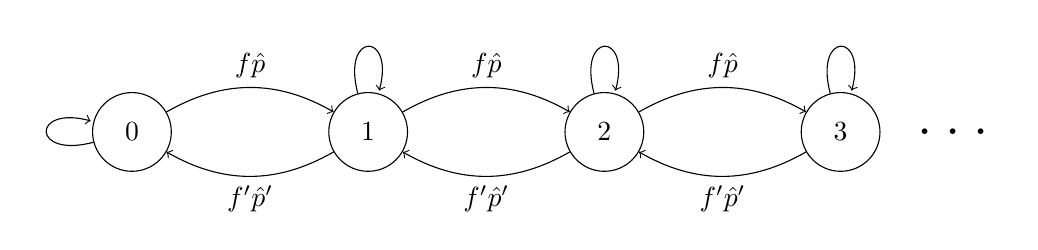
\begin{tikzpicture}
    % Define the nodes
    \node[draw, circle,minimum size=1cm] (s0) at (0,0) {0};
    \node[draw, circle,minimum size=1cm] (s1) at (3,0) {1};
    \node[draw, circle,minimum size=1cm] (s2) at (6,0) {2};
    \node[draw, circle,minimum size=1cm] (s3) at (9,0) {3};
    
    \node at (10.5,0) {\Huge\dots};
    % Arrows to the next state (curved up)
    
    \draw[->] (s0) to[bend left] node[midway, above] {$f\hat{p}$} (s1);
    \draw[->] (s1) to[bend left] node[midway, above] {$f\hat{p}$} (s2);
    \draw[->] (s2) to[bend left] node[midway, above] {$f\hat{p}$} (s3);

    % Arrows to the previous state (curved down)
    \draw[->] (s1) to[bend left] node[midway, below] {$f'\hat{p}'$} (s0);
    \draw[->] (s2) to[bend left] node[midway, below] {$f'\hat{p}'$} (s1);
    \draw[->] (s3) to[bend left] node[midway, below] {$f'\hat{p}'$} (s2);

    % Self-loop arrows
    \draw[->] (s0) edge[loop left] node[left] {} (s0);
    \draw[->] (s1) edge[loop above] node[above] {} (s1);
    \draw[->] (s2) edge[loop above] node[above] {} (s2);
    \draw[->] (s3) edge[loop above] node[right] {} (s3);
\end{tikzpicture}
\caption{Markov chain with queue length as states as observed at the slot boundary for an ARQ scheme. The transition probabilities, except the self-loop probabilities, are shown.}
\label{fig:markovChain_modified}
\end{figure*}


\subsubsection{Steady state probabilities}
We now focus on determining the steady-state probabilities (SSP) of the queue. Rather than directly finding the SSP of the initial Markov chain, we bound it using the SSP of a modified Markov chain representing an \textit{immediate feedback scenario} with $\delta = \ddecod = 0$, which is mathematically more tractable.

In such a scenario, the retransmission happens in the immediate next slot. One can alternatively consider that the departure occurs with a probability of $1-p$ instead of $1$, and there is no retransmission scheduled. 
The events between two state observations are an arrival at the start of the slot and a departure at the end of the slot with probabilities $f$ and $1-p$, respectively. 
Thus, the transition from state $q$ to $q+1$ comes with a probability $fp$, larger than $f\hat{p}$. 
Therefore, the CCDF of the queue length of this adapted Markov chain stochastically dominates that of the Markov chain from \ref{fig:markovChain_modified}. We will elaborate on this soon and use it to bind the violation probability of the wait delay. 

Let $\pi_i$ denote the steady-state probability of the adapted Markov chain. Lemma~\ref{lemma_arq_queue} provides the CCDS of the queue length.

\begin{lemma}\label{lemma_arq_queue}
    The CCDF of the queue length $Q$ is given by:
    \begin{equation}
        \mathbb{P}\left(Q>q\right) = \left(\dfrac{fp}{(1-f)(1-p)}\right)^{q+1}\label{eq:secARQ_QueueCCDF}
    \end{equation}
\end{lemma}
\begin{proof}
 \begin{align*}
    \pi_0 &= (1-fp)\pi_0 + f'p'\pi_1, \\
    \Rightarrow \pi_1 &= \dfrac{fp}{f'p'}\pi_0.\\
    \pi_1 &= fp\pi_0+ (1-fp-f'p')\pi_1+ f'p'\pi_2, \\
    \Rightarrow \pi_2 &= \dfrac{fp}{f'p'}\pi_1,\\
     &=  \left(\dfrac{fp}{f'p'}\right)^2\pi_0.
\end{align*}
Continuing with the same steps, we get
\begin{align*}
    \!\pi_i &= \left(\dfrac{fp}{f'p'}\right)^{i}\pi_0,\,\forall i\geq0,
    \intertext{that is,}
\!\pi_i &= \left(\dfrac{fp}{(1-f)(1-p)}\right)^{i}\!\!\left(1-\dfrac{fp}{(1-f)(1-p)}\right)\!,\forall i\geq0.\numberthis\label{eq:secARQ_ssp}
\end{align*}
Let $Q$ be the random variable denoting the queue length in the immediate feedback scenario, the distribution of which is given in \eqref{eq:secARQ_ssp}. Thus,
\begin{align*}
    \mathbb{P}\left(Q>q\right)&=\left(1-\dfrac{fp}{(1-f)(1-p)}\right)\\
    &\qquad\qquad\quad\sum_{i=q+1}^{\infty}\left(\dfrac{fp}{(1-f)(1-p)}\right)^{i},\,\forall i\geq0.\\
    &=\left(\dfrac{fp}{(1-f)(1-p)}\right)^{q+1}.
\end{align*}   
\end{proof}


% \paragraph*{Stability}
Observe that the queue is stable if the arrival rate does not exceed the departure rate, i.e. if $f \leq 1 - p$ or equivalently if $\frac{p}{1-f} \leq 1$. This can also be derived by computing the expected queue length $\Bar{\pi}$:
\begin{align*}
    \Bar{\pi} &=\left(1-\dfrac{fp}{(1-f)(1-p)}\right)\sum_{i=0}^{\infty}i\left(\dfrac{fp}{(1-f)(1-p)}\right)^{i},\\
    &=\left(1-\dfrac{fp}{(1-f)(1-p)}\right)\frac{(1-f)(1-p)}{(1-f-p)^2}fp,\\
    &=\frac{fp}{1-f-p},
\end{align*}
which implies stability when:
\begin{equation}
    \frac{p}{1-f}\leq1.\numberthis\label{eq:secARQ_zerofdbk_stability}
\end{equation}


\subsection{Wait delay}
It is clear from \eqref{eq:secARQ_QueueCCDF} that the queue length distribution of the immediate feedback scenario with PER $p$ stochastically dominates the queue length distribution of a delayed feedback scenario with a PER $\hat{p} < p$ in a first-order stochastic dominance sense~\cite{whang2019econometric}.


Let $\dwait\vert Q$ be the wait delay, conditioned on the queue length. Thus, 
\begin{align*}
    \mathbb{P}(\dwait =k)&=\sum_q\,\pi_q\mathbb{P}(\dwait ={k}\vert Q=q).
\end{align*}
As the wait delay increases with queue size, the stochastic dominance of the queue length of the delayed feedback scenario also implies the stochastic dominance of the corresponding wait delay. This will also become evident from Lemma~\ref{lemma_arq_wait}, where the upper bound, which is the CCDF of the wait delay with immediate feedback, decreases as the PER decreases. 
This upper bound is found to be sufficiently tight from simulations. This is because, unlike the service delay, the wait delay measured from arrival to the first transmission is largely unaffected by the feedback.


Recall that the sum of i.i.d. geometric random variables follows a negative binomial distribution\cite{johnson2005univariate}. 
For $X_{q}$ representing such a sum, the probability mass function is given by:
\begin{equation}
    \mathbb{P}(X_{q}=k)=\dfrac{(k-1)!}{(q-1)!(k-q)!}(1-p)^qp^{k-q}.\label{eq:secARQ_geoSum}
\end{equation}
% We now bound $\dwait$ by marginalizing the conditional distribution over steady-state queue probabilities.
 % \todo[inline]{Discuss more or prove mathematically the stochastic dominance?}
\begin{lemma}\label{lemma_arq_wait}
    The CCDF of the wait delay is given by:
    \begin{equation}
  \mathbb{P}(\dwait >k) \leq\frac{f}{1-p}\left(\frac{p}{1-f}\right)^{k+1}.\label{eq:secARQ_waitdelay} 
    \end{equation}
\end{lemma}
\begin{proof}
For the immediate feedback scenario, the number of transmissions attempted by a packet in the queue is distributed geometrically. Thus, $\mathbb{P}(D_w\vert Q)$ is given by the sum of $Q$ iid geometrically distributed random variables. We have,
\begin{align*}
\mathbb{P}(\dwait\!>\!j)&\leq 1\!-\!\left(\pi_0+\sum_{k=1}^{j}\sum_{q=1}^{k}\pi_q\,\mathbb{P}(D_w=k\vert Q=q)\right),\,\forall j\geq0.
\end{align*}
 Here, $\pi_0$ represents an empty queue. Let $Z(k)$ denote the inner sum. Expanding with \eqref{eq:secARQ_geoSum}, we have:
 \begin{equation}
Z(k)=\sum_{q=1}^{k}\pi_q\dfrac{(k-1)!}{(q-1)!(k-q)!}(1-p)^qp^{k-q},\,\forall k\geq1.
 \end{equation}
\begin{align*}
&=\sum_{q=1}^{k} 
\left( \frac{f \, p}{(1 - f) \, (1 - p)} \right)^q 
\left(1 - \frac{f \, p}{(1 - f) \, (1 - p)} \right)\\&\hspace{8em}
\left( \frac{(k - 1)!}{(k - q)!\,(q - 1)!} \right)
(1 - p)^q \, p^{k - q},\\
&=\left(1 - \frac{f \, p}{(1 - f) \, (1 - p)} \right)\sum_{q=0}^{k-1} 
\left( \frac{f \, p}{(1 - f) \, (1 - p)} \right)^{q+1} \\&\hspace{6em}
\left( \frac{(k - 1)!}{(k - q-1)!\,(q)!} \right)
(1 - p)^{q+1} \, p^{k - q-1},\\
% &=\left(1 - \frac{f \, p}{(1 - f) \, (1 - p)} \right)\sum_{q=0}^{k-1} 
% p^{q+1}\left( \frac{f}{(1 - f)} \right)^{q+1} 
% \left( \frac{(k - 1)!}{(k - q-1)!\,(q)!} \right) p^{k - q-1}\\
&=\left(1 - \frac{f \, p}{(1 - f) \, (1 - p)} \right)
p^{k}
\sum_{q=0}^{k-1} 
\left( \frac{f}{1 - f} \right)^{q+1}\\&\hspace{13em}
\left( \frac{(k - 1)!}{(k - 1 -q)!\,(q)!} \right),\\
&=\left(1 - \frac{f \, p}{(1 - f) \, (1 - p)} \right)
p^{k}\left( \frac{f}{1 - f} \right)
% \\&\hspace{12.5em}
\sum_{q=0}^{k-1} {\binom{k-1}{q}}
\left( \frac{f}{1 - f} \right)^{q},\\
&=\left(1 - \frac{f \, p}{(1 - f) \, (1 - p)} \right)
p^{k}\left( \frac{f}{1 - f} \right)
% \\&\hspace{15.5em}
\left(1+ \frac{f}{1 - f} \right)^{k-1},\\
% &=f\,\left( \frac{p}{1 - f} \right)^{k}
% \left(1 - \frac{f \, p}{(1 - f) \, (1 - p)} \right)\\
% \Rightarrow\mathbb{P}(\dwait >k) &= 1-\left(\pi_0+\sum_{i=1}^{k}\mathbb{P}(\dwait =k)\right)
&=f\,\left( \frac{p}{1 - f} \right)^{k}
\frac{1-f-p}{(1 - f) \, (1 - p)}.
\end{align*}
\begin{equation*}
 \Rightarrow\mathbb{P}(\dwait >j) \leq 1-\left(\pi_0+\sum_{k=1}^{j}Z(k)\right),  
\end{equation*}
\begin{align*}
% \Rightarrow\mathbb{P}(\dwait >j) &\leq 1-\left(\pi_0+\sum_{k=1}^{j}Z(k)\right)\\
&=1-\left(\pi_0+\sum_{k=1}^{j}f\,\left( \frac{p}{1 - f} \right)^{k}
\frac{1-f-p}{(1 - f) \, (1 - p)}\right),\\
% \Rightarrow\mathbb{P}(\dwait >j) &= 1-\left(\frac{1-f-p}{(1 - f) \, (1 - p)}+\sum_{k=1}^{j}f\,\left( \frac{p}{1 - f} \right)^{k}
% \frac{1-f-p}{(1 - f) \, (1 - p)}\right)\\
% \Rightarrow\mathbb{P}(\dwait >j) &= 1-\left(\frac{1-f-p}{(1 - f) \, (1 - p)}\right)\left(1+\sum_{k=1}^{j}f\,\left( \frac{p}{1 - f} \right)^{k}\right)\\
 &= 1-\left(\frac{1-f-p}{(1 - f) \, (1 - p)}\right)\left(1 + f\sum_{k=1}^{j}\left( \frac{p}{1 - f} \right)^{k}\right),\\
 &= 1-\left(\frac{1-f-p}{(1 - f) \, (1 - p)}\right)\\&\hspace{6em}\left(1 + \frac{fp}{1-f-p}\left(1-\left(\frac{p}{1-f}\right)^j\right)\right),\\
&= 1-\left(1-f-p+fp-fp\left(\frac{p}{1-f}\right)^j\right)\\&\hspace{13.5em}\left(\frac{1}{(1 - f) \, (1 - p)}\right),\\
&=\frac{fp}{(1-f)\,(1-p)}\left(\frac{p}{1-f}\right)^j,\\
&=\frac{f}{1-p}\left(\frac{p}{1-f}\right)^{j+1}.
\end{align*}
\begin{equation}
    \Rightarrow\mathbb{P}(\dwait >k) \leq\frac{f}{1-p}\left(\frac{p}{1-f}\right)^{k+1}.\nonumber
\end{equation}
\end{proof}

\subsection{Delay Violation Probability}\label{NoIR_dvp}
To get the DVP, we combine the upper bound of $\dwait$ with the service delay. The service delay is geometrically distributed based on the failure probability at the corresponding attempt, with values depending on $\delta$. It is given by:
\begin{align}
    \mathbb{P}\left(\dserv =k(\ddecod+1)+\delta(k-1)\right) &= p^{k-1}(1-p).\label{eq:secARQ_servDelay}\\
    \mathbb{P}\left(\dserv >k(\ddecod+1)+\delta(k-1)\right) &= p^{k}.\nonumber
\end{align}
Recall $k_d$ defined as the maximum number of transmissions possible before the service delay alone exceeds the delay target:
\begin{align}
    k_d\,\coloneqq& \underset{i}{Max}\,\left\{\,i:i(\ddecod+1)+(i-1)\delta\leq\left\lfloor\frac{d}{T}\right\rfloor\,\right\}\nonumber\\
    =&\left\lfloor\frac{\frac{d}{T}+\delta}{\delta+\ddecod+1}\right\rfloor.\label{eq:secARQ_kd}
\end{align}
\begin{theorem}\label{theorem_arq_dvp}
The DVP of the ARQ scenario for a delay target $d$ is given by:
\begin{multline}
\mathbb{P}(\dtot >d)\leq p^{ k_d } \\-  
\dfrac{f\,\left(\frac{p}{1-f}\right)^{  \left\lfloor\nicefrac{d}{T}\right\rfloor +\delta}
\left(1-p^{ k_d }\left(\frac{p}{1-f}\right)^{- k_d (1+\delta+\ddecod)}
\right)}
{1-f-\left(\frac{p}{1-f}\right)^{\delta+\ddecod}}.\numberthis\label{dvpbound}
\end{multline}
\end{theorem}
\begin{proof}
We have,
\begin{align*}
\mathbb{P}(\dtot >d)&\leq \sum_{i}\mathbb{P}(\dserv =i)\mathbb{P}(\dwait >d-i),\\
% &= p^{k_d} + \sum_{i=1}^{{ k_d }} (1 - p) p^{i - 1} \left( \sum_{k = 1 + \left\lfloor\nicefrac{d}{T}\right\rfloor - (i + (i - 1) {\delta})}^{\infty}f\,\left( \frac{p}{1 - f} \right)^{k}
% \frac{\left(1-f-p\right)}{(1 - f) \, (1 - p)}\right)
&= p^{k_d} + \sum_{i=1}^{{ k_d }} (1 - p) p^{i - 1}
\\&\hspace{2.5em}\left( \frac{f}{1-p}\left(\frac{p}{1-f}\right)^{1 + \left\lfloor\nicefrac{d}{T}\right\rfloor - \big(i(\ddecod+1) + (i - 1) {\delta}\big)}\right).
\end{align*}
The first term corresponds to the probability that the service delay alone exceeds the target. The second term accounts for a successful transmission at the $i^{\mathrm{th}}$ attempt with a service delay of $i(\ddecod+1) + (i-1)\delta$, along with all possible wait delays from \eqref{eq:secARQ_waitdelay} that in combination violate the delay target.
\begin{multline}
    \Rightarrow\mathbb{P}(\dtot >d) \leq p^{k_d} + 
f\left(\frac{p}{1-f}\right)^{1 + \left\lfloor\nicefrac{d}{T}\right\rfloor + \delta}\,
\\\sum_{i=1}^{{ k_d }}p^{i - 1} \left(\frac{p}{1-f}\right)^{-i(1+\delta+\ddecod)}
\end{multline}
\begin{align*}
&= p^{k_d} + 
f\left(\frac{p}{1-f}\right)^{1 + \left\lfloor\nicefrac{d}{T}\right\rfloor + \delta}\,
\\&\hspace{10.5em}\sum_{i=0}^{{ k_d -1 }} p^{i} \left(\frac{p}{1-f}\right)^{-(i+1)(1+\delta+\ddecod)}\\
&= p^{k_d} + 
f\left(\frac{p}{1-f}\right)^{1 + \left\lfloor\nicefrac{d}{T}\right\rfloor + \delta}\,
\left(\frac{p}{1-f}\right)^{-(1+\delta+\ddecod)}\,
\\&\hspace{10.5em}\sum_{i=0}^{{ k_d -1 }} p^{i} \left(\frac{p}{1-f}\right)^{-i(1+\delta+\ddecod)}\\
&= p^{k_d} + 
f\left(\frac{p}{1-f}\right)^{ \left\lfloor\nicefrac{d}{T}\right\rfloor-\ddecod}\,
\sum_{i=0}^{{ k_d -1 }} p^{i} \left(\frac{p}{1-f}\right)^{-i(1+\delta+\ddecod)}\\
% &= p^{k_d} + 
% f\left(\frac{p}{1-f}\right)^{ \left\lfloor\nicefrac{d}{T}\right\rfloor}\,
% \frac{1-\left(p\left(\frac{p}{1-f}\right)^{-(1+\delta)}\right)^{k_d}}{1-\left(p\left(\frac{p}{1-f}\right)^{-(1+\delta)}\right)}\\
&= p^{k_d} + 
f\left(\frac{p}{1-f}\right)^{ \left\lfloor\nicefrac{d}{T}\right\rfloor-\ddecod}\,
\frac{1-p^{k_d}\left(\frac{p}{1-f}\right)^{-k_d(1+\delta+\ddecod)}}{1-p\left(\frac{p}{1-f}\right)^{-(1+\delta+\ddecod)}}
% &= p^{ k_d } +  
% \dfrac{f\,\left(\frac{p}{1-f}\right)^{  \left\lfloor\nicefrac{d}{T}\right\rfloor +\delta}
% \left(1-p^{ k_d }\left(\frac{p}{1-f}\right)^{- k_d (1+\delta)}
% \right)}
% {\left(\frac{p}{1-f}\right)^{\delta}\left(1-p\left(\frac{p}{1-f}\right)^{-(1+\delta)}\right)}\\
\end{align*}
\begin{multline}
    \Rightarrow\mathbb{P}(\dtot >d)\leq p^{ k_d } \\-  
\dfrac{f\,\left(\frac{p}{1-f}\right)^{  \left\lfloor\nicefrac{d}{T}\right\rfloor +\delta}
\left(1-p^{ k_d }\left(\frac{p}{1-f}\right)^{- k_d (1+\delta+\ddecod)}
\right)}
{1-f-\left(\frac{p}{1-f}\right)^{\delta+\ddecod}}
\end{multline}
\end{proof}
% \todo[inline]{Outro?}








\section{HARQ: Incremental Redundancy}\label{sec:harq}
In this section, we consider the HARQ scenario with incremental redundancy. 
As discussed earlier, we assume that the coded packet length for all transmissions remains constant, thereby attaining the maximum increment in redundancy with reach retransmission. 
The PER is represented by the vector $\Vec{p}=\begin{bmatrix}p_1 & p_2 & \dots & p_M\end{bmatrix}$. We assume a maximum of $M$ transmissions and a maximum of $Q_{\mathrm{max}}$ parallel HARQ processes. Typically, $M=4$, and $Q_{\mathrm{max}}$ is 8 or 16 in real HARQ implementations.
\begin{table}[b]
\centering
\renewcommand{\arraystretch}{1.25}
\renewcommand{\arraystretch}{1.25}
\begin{tabular}{|l|l|l|l|l|}
\hline
\multicolumn{1}{|c|}{\multirow{2}{*}{State}} & \multicolumn{1}{c|}{\multirow{2}{*}{Next state}} & \multicolumn{1}{c|}{Range} & \multicolumn{1}{c|}{Range} & \multicolumn{1}{c|}{Proba-} \\
\multicolumn{1}{|c|}{}                       & \multicolumn{1}{c|}{}                            & \multicolumn{1}{c|}{$(q)$}   & \multicolumn{1}{c|}{$(m)$}   & \multicolumn{1}{c|}{bility} \\ \hline
$(0,1)$                                      & $(0,1)$                                          &   -                        &   -                        & $1-fp_1$                    \\
$(0,1)$                                      & $(1,2)$                                          &   -                        &   -                        & $fp_1$                      \\
$(q,m)$                                      & $(q,m+1)$                                        & $[1,\qmax)$                & $[1,M)$                    & $f'p_m$                     \\
$(q,m)$                                      & $(q+1,m+1)$                                      & $[1,\qmax)$                & $[1,M)$                    & $fp_m$                      \\
$(q,m)$                                      & $(q,1)$                                          & $[1,\qmax]$                & $[1,M)$                    & $fp_m'$                     \\
$(q,m)$                                      & $(q-1,1)$                                        & $[1,\qmax]$                & $[1,M)$                    & $f'p_m'$                    \\
$(q,M)$                                      & $(q,1)$                                          & $[1,\qmax]$                &    -                       & $f$                         \\
$(q,M)$                                      & $(q-1,1)$                                        & $[1,\qmax]$                &    -                       & $f'$                        \\
$(\qmax ,m)$                                 & $(\qmax ,m+1)$                                   &        -                   & $[1,M)$                    & $p_m$                       \\ \hline
\end{tabular}
\caption{Non-zero probabilities of the transition probability matrix $P$ for a given $q$ and $m$. State number $s=qM+m$ for the state $(q,m)$. $f'=1-f,\;p_m'=1-p_m.$}
\label{table:IR}
\end{table}

To compute the DVP, we proceed similarly to the previous section by combining the wait delay and service delay, which are computed separately. 
We propose an algorithmic approach to compute the wait delay, as this is more suited for HARQ with a relatively small $M$, $\qmax$, and a non-iid PER across the retransmissions.
% Adapting the ARQ queuing model to include maximum retransmissions and non-identical PERs is not straightforward, so we propose an algorithmic approach to address this.
As before in Section~\ref{sec:arq}, we bound the wait delay bound using the immediate feedback scenario where the retransmissions happen in the immediate next slot.
We now construct the Markov chain transition probability matrix of this scenario.

\subsection{Queueing Model}
We define $(\qmax+1)M$ states, denoted by the tuple $(q,m)$, where $0 \leq q \leq Q_{\mathrm{max}}$ and $1 \leq m \leq M$, measured at the slot boundary. The states represent the current queue length $q$ (observed by a newly arriving packet) and the transmission number $m$ of the packet that will be transmitted in the next slot. 
For example, the state $(3,2)$ indicates that the queue length of $3$ and the packet to be transmitted has already failed once. 
% In this section, we directly for the adapted model discussed Section~\ref{sec:arq}, where we look at the Markov chain whose steady state distribution dominates the actual queue distribution.


The non-zero transition probabilities for all states are given in Table~\ref{table:IR}. For ease in constructing and using the transition probability matrix $P_{(q+1)M\times (q+1)M}$, we number the states as $s=1,2,\dots,(qM+m),\dots,(q+1)M$. The states $(0,m), m \geq 2$ are never reached and are included for uniformity and simplicity. These states are defined with a self-loop probability of 1 and have a steady-state probability of 0.

% \begin{table*}[t]
% \centering
% \begin{tabular}{|l|l|l|l|l|}
% \hline
% State                  & Next State               & Range ($q$)                & Range ($m$)  & Probability \\ \hline
% $(0,1)$                & $(0,1)$                  &                            &              & $1-fp_1$    \\ \hline
% $(0,1)$                & $(1,2)$                  &                            &              & $fp_1$      \\ \hline
% $(q,m)$                & $(q,m+1)$                & $1\leq  q< \qmax $   & $1\leq m<M$  & $f'p_m$     \\ \hline
% $(q,m)$                & $(q+1,m+1)$              & $1\leq  q<\qmax $    & $1\leq m<M$  & $fp_m$      \\ \hline
% $(q,m)$                & $(q,1)$                  & $1\leq q\leq \qmax $ & $1\leq m< M$ & $fp_m'$     \\ \hline
% $(q,m)$                & $(q-1,1)$                & $1\leq q\leq \qmax $ & $1\leq m< M$ & $f'p_m'$    \\ \hline
% $(q,M)$                & $(q,1)$                  & $1\leq q\leq \qmax $ &              & $f$         \\ \hline
% $(q,M)$                & $(q-1,1)$                & $1\leq q\leq \qmax $ &              & $f'$        \\ \hline
% $(\qmax ,m)$ & $(\qmax ,m+1)$ &                            & $1\leq m< M$ & $p_m$       \\ \hline
% \end{tabular}
% \caption{Non-zero probabilities of the transition probability matrix $P$. State number $s=qM+m$ for the state $(q,m)$. $f'=1-f,\;p_m'=1-p_m.$}
% \label{table:IR}
% \end{table*}


The probabilities can be explained as follows: $f$ represents arrival, and $p_m$ represents the PER at the $m^{\mathrm{th}}$ attempt. For state $(0,1)$, an arrival and transmission failure lead to a transition to state $(1,2)$, while other possibilities result in a loop. In states with $m=M$, the PER becomes irrelevant because the packet is either successfully transmitted or discarded. Similarly, a packet is dropped when an arrival and transmission failure occurs at state $(Q_{\mathrm{max}},m)$ due to a queue overflow. For other states, the transitions follow the typical pattern: failures increase $m$, successes reset $m$ to 0, and arrivals/departures adjust the queue size based on the transmission outcome.

Once $P$ is constructed, the steady-state probabilities, denoted by $\Tilde{\pi}$, can be computed by finding the eigenvector of $P^T$ corresponding to the unit eigenvalue. This can be done using standard algorithms or by iterating $P$ until $P^i \approx P^{i+1}$, with the rows converging to the steady-state probabilities.

The steady-state probabilities $\Tilde{\pi}$ are for the modified Markov chain with $(Q_{\mathrm{max}}+1)M$ states. To obtain the steady-state probabilities ${\pi}$ for each queue length $q=1,2,\dots, Q_{\mathrm{max}}$, we sum the probabilities of all states with the same queue length but different $m$ values:
\begin{equation}
    \pi_q = \sum_{s=qM}^{(q+1)M}\Tilde{\pi}_s.
\end{equation}
We assume that $\qmax$ is chosen such that packet drops due to queue overflow are negligible, typical in a high-reliability setting. Otherwise, one could repeat with a larger $\qmax$. That being said, we do consider the drops emerging from packets reaching the retransmission limit of HARQ ($m=M$), which cannot be neglected.

\subsection{Wait Delay}
To compute the wait delay, we start by finding $f_W(k|q)$, the conditional wait probability given queue length $q$. We propose ALGORITHM~\ref{Alg:getWaitProbability} to compute this for a given $k,q,\Vec{p}$ and $M$ using combinatorics.
% recursively by summing $q$ i.i.d. random variables, each representing transmission attempts with probabilities $p_1, p_2, \dots, p_M$. 
% The wait delay is 0 if and only if the queue length is 0, so $f_W(0)~=~\pi_0$. 
The unconditional wait delay pmf is obtained by marginalizing the queue length probabilities:
\begin{equation}
    f_{\dwait}(k)=\mathbb{P}(\dwait=k) \leq \sum_{q=0}^{\infty}\pi_qf_W(k|q).\label{eq:secIR_waitDelay}
\end{equation}
\begin{algorithm}[t]
\caption{Recursive function \textit{getWaitProbability} to compute the conditional probability of wait delay of $k$ slots given a queuelength of $q$ packets. The global constant $M_0 = M$ in the first call of the recursion.}
\begin{algorithmic}[th]
% \State $M_0 \gets M$\Comment{$M_0$ is a global constant.}
\Function{getWaitProbability}{$k, q, \Vec{p}, M, M_0$}
    \If{$k == q$}
        \State\Return $(1 - \Vec{p}_1)^q$
        \Comment{$k=q\Rightarrow$ all success.}
    \ElsIf{$k < q$ \textbf{or} $k > M \cdot q$}
        \State\Return $0$
        \Comment{Out of range, $prob = 0$.}
    \EndIf
    \State $prob \gets 0$
    \State $N \gets \min(\text{floor}((k - q) / (M - 1)), q)$\
        \\\Comment{Max \#packets with max attempts $=M$.}
    \For{$n = 0$ \textbf{to} $N$}
        \State $numSeqs \gets \dbinom{q}{n}$
        \State $seqProbFail \gets \prod_{i=1}^{M-1}\Vec{p}_{i}$
        
        \If{$M == M_0$}
            \State $seqProbSucc \gets 1$
            \\\Comment{Handle discard case when $M = M_0$.}
        \Else
             \State $seqProbSucc \gets (1 - \Vec{p}_M)$
        \EndIf
        
        \State $seqProb\gets(seqProbFail \cdot seqProbSucc)^n$
        \State $subSeqProb \gets$ \Call{getWaitProbability}{}
        \State \qquad\qquad\qquad\qquad($k-Mn, q - n, \Vec{p}, M - 1, M_0$)
        \\\Comment{Recursion.}
        \State $prob \gets prob + numSeqs\!\cdot\!seqProb\!\cdot\!subSeqProb$
    \EndFor
    \State \Return $prob$
\EndFunction
\end{algorithmic}
\label{Alg:getWaitProbability}
\end{algorithm}






\subsection{Delay Violation Probability}
We now compute the distributions of the service delay, similar to Section~\ref{NoIR_dvp}. 
The service delay is determined by the PER vector and $k_d$, the maximum number of transmissions allowed before exceeding the delay target. 
Unlike \eqref{eq:secModel_Kd}, where we assumed infinite retransmissions, here we limit $k_d$ by $M$:
\begin{align}
k_{d}&=\min\left(M,\left\lfloor\frac{\nicefrac{d}{T}+\delta}{\delta+\ddecod+1}\right\rfloor\right),\label{eq:secIR_kd}\\
\mathbb{P}(\dserv>d)&=\prod_{i=1}^{k_{d}}p_i.\label{eq:secIR_servDelay}
\end{align}
% To compute the queue length or wait time probabilities in practice, we terminate the algorithm once the probability reaches zero (or a sufficiently small value), as these probabilities decrease monotonically. 
Let $k_{d-kT}$ denote the $k_d$ for the delay target $d-kT$. 
\begin{align*}
    k_{d-kT}&=\min\left(M,\left\lfloor\frac{\nicefrac{(d-kT)}{T}+\delta}{\delta+1}\right\rfloor\right),\nonumber\\
    &=\min\left(M,\left\lfloor\frac{\nicefrac{d}{T}-k+\delta}{\delta+\ddecod+1}\right\rfloor\right).
\end{align*}

Finally, the total DVP is computed as before in Section~\ref{NoIR_dvp}, using the wait delay and service delay violation probabilities:
\begin{align}
    \mathbb{P}(\dtot>d) &=\sum_k \mathbb{P}(\dwait=k)\mathbb{P}(\dserv>d-k)\nonumber\\
    % \sum_kf_{D_w}(k)\prod_{i=1}^{ \min\left(M,1 + \left\lfloor\frac{\nicefrac{d}{T}-1}{\delta+1}\right\rfloor\right)}p_i
    &\leq\sum_kf_{\dwait}(k)\prod_{i=1}^{k_{d-kT}}p_i.\label{eq:secIR_totDelay}
\end{align}
% \todo[inline]{Outro?}
% \section{Deterministic Arrivals}\label{sec:detArr}
\todo[inline]{Remove this, or move to an appendix?}
In this section, we look at a URLLC-enabled system where the arrivals are deterministic with a cycle time $c$. This could, for instance, be a UE with sensor capabilities that samples the environment and send the data to the gNB. 
The DVP is straightforward when $c\geq M\cdot\text{RTT}$ and resembles the BAR model discussed as a warm-up in Section~\ref{sec:model}, where the queue is never formed.
Otherwise, a numerical approach similar to HARQ is required.
\subsection{Queing Model}
We observe the queue state only at the boundary of every $c$ slots. Between observations, exactly one packet arrives, and up to $c$ packets may succeed. A transition from state $q$ to state $(q-k+1)$ occurs when exactly $k$ slots succeed, where $0 \leq k \leq \min(q+1, c)$, with the following probabilities:
\begin{align}
\mathbb{P}(q \to q-k+1) &= \binom{c}{k} (1-p)^k p^{c-k},\;q\geq c,\,0\leq k \leq c,\label{eq:secDet_transProb1}\\   
\mathbb{P}(q \to q-k+1) &= \binom{c}{k} (1-p)^k p^{c-k},\;q<c,\,0\leq k\leq q,\label{eq:secDet_transProb2}\\  
\mathbb{P}(q \to 0) &= \sum_{k=q+1}^{c}\binom{c}{k} (1-p)^k p^{c-k},q<c.\label{eq:secDet_transProb3}
\end{align}
When $q < c$, a transition to state 0 is realized by summing the probabilities for multiple outcomes, as shown in \eqref{eq:secDet_transProb2} and \eqref{eq:secDet_transProb3}.
% For easier understanding, this single expression can be split into multiple cases as follows:
% \begin{itemize}
% \item For state $q = 0 $:
% \begin{itemize}
%     \item $\mathbb{P}(0 \to 1) = p^c$
%     \item $ \mathbb{P}(0 \to 0) = 1-p^c$
% \end{itemize}
% \item For states $1\leq q\leq c-1$:
% \begin{itemize}
%     \item $\mathbb{P}(q \to q+1) = p^c$
%     \item$\mathbb{P}(q \to q-(k-1)) = \binom{c}{k} (1-p)^k p^{c-k},\,\forall k\leq q$
%     \item $\mathbb{P}(q \to 0) =\sum_{k=q+1}^{c}\binom{c}{k} (1-p)^k p^{c-k}$
% \end{itemize}
% \item For states $q\geq c$:
% \begin{itemize}
%     \item     $\mathbb{P}(q \to q-(k-1)) = \binom{c}{k} (1-p)^k p^{c-k}$
% \end{itemize}
% \end{itemize}

Define $(x)^+ \coloneqq \mathrm{max}(0, x)$. The steady-state probabilities $\pi_q$ for $q \geq 0$ can be computed by solving the following equations:
% \begin{align*}
%         \pi_0 &=\sum_{k=1}^{\min(1+c, c)} \pi_{k-1} \binom{c}{k} (1-p)^k p^{c-k}\\
%         \pi_1 &= \pi_0 p^c + \pi_1 \binom{c}{1} (1-p) p^{c-1} + \sum_{k=3}^{\min(2+c, c)} \pi_{k-1} \binom{c}{k} (1-p)^k p^{c-k}\\
%         \pi_q &= \pi_{q-1} p^c + \pi_q \binom{c}{1} (1-p) p^{c-1} + \sum_{j=q+1}^{\min(+1+c, c)} \pi_{j-1} \binom{c}{j} (1-p)^j p^{c-j}
% \end{align*}
\begin{align*}
\pi_q &=\sum_{k=0}^{c}\binom{c}{k}\,(1-p)^k p^{c-k}\;\pi_{(q+k-1)^{+}}\\
&=p^c\,\pi_{(q-1)^+}\;+\;\sum_{k=1}^{c}\binom{c}{k}\,(1-p)^k p^{c-k}\,\pi_{q+k-1}
\intertext{That is,}
\pi_q &=\begin{cases}
    &p^c\,\pi_{0}\;+\;\sum_{k=1}^{c}\binom{c}{k}\,(1-p)^k p^{c-k}\,\pi_{q+k-1},\\
    &\hspace{16em}\quad if\;q=0,\\ 
    &p^c\,\pi_{q-1}\;+\;\sum_{k=1}^{c}\binom{c}{k}\,(1-p)^k p^{c-k}\,\pi_{q+k-1},\\
    &\hspace{16em}\quad if\;q>0,
\end{cases}
\end{align*}
where, $\pi_q=0,\,\forall q>\qmax.$
We Solve this by choosing an appropriate maximum queue size $Q$ and finding $\{\pi_q\}$ using either the equations or the transition probability matrix. If $\pi_{Q_{\max}}$ is not sufficiently small, we repeat the process with a larger $Q_{\max}$. 

With the queue length statistics available, finding the service delay and wait delay conditioned on the queue length follows the same steps as in previous sections. We marginalize these over the steady state queue length probabilities to get the unconditioned wait and service delays and then compute the DVP.

Recall that the comparison between deterministic arrivals and random arrivals is interesting. Even if the average arrival rate is the same, the queues can be different. How different, of course, depends on the parameters. This is because the variance of the inter-arrival time in terms of a queue with deterministic arrivals is zero and, hence, does not result in larger queues due to burst arrivals. Thus the average queue length -- and as a result, wait times -- of a queue with deterministic arrivals are typically smaller than that of a queue with random arrivals with the same arrival and service rates. 



\section{Numerical Evaluation}\label{sec:simulations}
We begin this section on numerical evaluation by detailing the parameter configuration, including default settings, MCS selection processes, and PER computation methods. 
We then compare the proposed ARQ and HARQ DVP evaluation schemes with the state-of-the-art IF approximation, showing the importance of not ignoring the decoding and feedback delay. 
Following this, we study key DVP trends across varying system parameters by examining the impact of RTT, resource allocation, and arrival rate on the evaluated DVP. Throughout this section, we consider a persistent ARQ with unlimited retransmissions and queue size, i.e., $M = \qmax = \infty$ and a typical HARQ configuration of $M = 4$ and $\qmax = 16$. 

\subsubsection*{Parameter Configuration}
We proposed DVP evaluation for ARQ and HARQ across various system parameters, leading to numerous permutations of parameter settings and illustrations. However, for clarity and conciseness, we limit our evaluation to key configurations.
Since incorporating decoding and feedback delays and supporting parallel ARQ/HARQ processes is the key novelty of this work, we choose RTT and the delay threshold $d$, which directly influences the DVP. 
We consider allocated $\nrb$ and packet length to highlight resource allocation implications and the arrival frequency $f$ to study system throughput. 
Default parameter values and ranges are listed in TABLE~\ref{table:params}. We set $\hvar=1$, $\gamma = 10$ dB, and $V=1$ as $\vert V-1\vert<0.0414,\,\forall\,\text{SNR}>4.1$ dB in an AWGN channel~\cite{polyanskiy2010FBL}. In each figure, a subset of parameters is varied, and the default values are used for the rest.

While some parameters like $\nrb$ are configurable, others are application-specific or come from the device capabilities. For example, \cite{3gpp.22.261} outlines KPI requirements for various applications. Similarly, RTT depends on factors such as decoding capabilities, feedback scheduling delays, and priority levels assigned by the gNB.
To ensure broad applicability, we use parameters within a typical range and present results independent of specific applications or scenarios.
\begin{table}[t]
\centering
\renewcommand{\arraystretch}{1.25}
\begin{tabular}{|l|l|l|}
\hline
Parameter             & Default value  & Range                                                                                                                            \\ \hline
$n$                   & 100$\times$8 b & $\{30, 50, 100, 200\}\times8$ b                                                                                                  \\
$\eta_{\mathrm{min}}$ & 0.2344         & -                                                                                                                                \\
$\eta_{\mathrm{max}}$ & 5.5547         & -                                                                                                                                \\
$\nrb$                & 10             & $\left\{\left\lceil\frac{n}{180\eta_{\mathrm{max}}}\right\rceil,\left\lceil\frac{n}{180\eta_{\mathrm{min}}}\right\rceil\right\}$ \\
$\snr$                & 10 dB          & -                                                                                                              \\
$\ddecod$             & 1 slot         & -                                                                                                                                \\
$\delta$              & 2 slots        & -                                                                                                                                \\
RTT                   & 4 slots        & $[1,7]$ slots                                                                                                                    \\
$d$                   & 8.5 ms         & $[2, 20]$ ms                                                                                                                     \\
$f$                   & $\frac{1}{3}$  & -                                                                                                                                \\
$\hvar$               & 1              & -                                                                                                                                \\
$V$                   & 1              & -                                                                                                                                \\ \hline
\end{tabular}
\caption{Default values and range of important parameters.}
\label{table:params}
\end{table}
\begin{figure}[b]
\centering
\includegraphics[width=0.98\linewidth]{Figures/comparison.eps}
\caption{Performance comparison of the proposed DVP evaluation schemes with the immediate feedback (IF) schemes for default configuration. The simulated DVP is also shown.}
\label{fig.Comparison}
\end{figure}
\begin{figure*}[t]
\centering
\begin{subfigure}[t]{0.49\linewidth}
\centering
\includegraphics[width=\textwidth]{Figures/blerVsNrb_vsRtt.eps}
\caption{DVP vs. $\nrb$ for different RTT. $d=8.5$ ms.}
\label{fig:Sim_dvp-nrb-rtt}
\end{subfigure}
\begin{subfigure}[t]{0.49\linewidth}
\centering
\includegraphics[width=\textwidth]{Figures/blerVsNrb_vsDelayTarget.eps}
\caption{DVP vs. $\nrb$ for different target delay $d$. RTT $=4$ slots.}
\label{fig:Sim_dvp-nrb-d}
\end{subfigure}
\caption{DVP vs. allocated $\nrb$ per slot for different delay parameters, namely RTT and $d$.}
\label{fig:Sim_dvp-nrb-nAndRtt}
\end{figure*}

Now, we move on to the MCS selection mechanism. 
The MCS selection follows 3GPP standards~\cite{3gpp.38.214}, where we choose an MCS index from 0 to 28, and obtain the modulation order, coding rate and spectral efficiency $\eta$ corresponding to it.
This range of MCS corresponds to a lower and upper limit of possible $\nrb$ for a given uncoded packet length $n$.
To minimize DVP for a given $\nrb$, the smallest MCS with $180\nrb\eta\geq n$ is chosen, that is, an MCS capable of supporting $n$ bits on $\nrb$ resources. 

We compute PER for ARQ and HARQ using \eqref{eq:secModel_perARQ} and \eqref{eq:secModel_perHARQ}, respectively. 
For DVP calculation, we use \eqref{dvpbound} for ARQ and ALGORITHM~\ref{Alg:getWaitProbability} with \eqref{eq:secIR_waitDelay} and \eqref{eq:secIR_totDelay} for HARQ. Note that we observe the DVP changing in steps at various points in all figures. This results from the finite and discrete nature of MCS selection and RB allocation in the 5G standard. 


\subsubsection*{Performance Comparison}
To evaluate performance, we compare the proposed methods with state-of-the-art single-server models, which are accurate only under the assumption of zero decoding and feedback delays, thereby eliminating the need for multiple processes. In this section, these models are referred to as the immediate feedback models (IF), where feedback is assumed to be available immediately after the transmission slot, effectively setting RTT to one slot.
The IF serves as the benchmark because the key novelty of this work lies in addressing the unrealistic assumptions of zero RTT and single-process ARQ/HARQ implementations.
We use two IF benchmarks, ARQ-IF and HARQ-IF, derived by setting $\ddecod = \delta = 0$ in the ARQ and HARQ schemes, respectively.


In Fig.~\ref{fig.Comparison}, we present the DVP for ARQ, HARQ, and IF under the default parameter settings, with the HARQ results validated using an event-based numerical simulation in MATLAB. The simulation confirms that, under the model assumptions, HARQ accurately computes the DVP across different values of $\nrb$, reflecting a realistic 5G scenario.
Next, we observe that ARQ consistently produces a worse DVP than HARQ, as expected, due to the absence of incremental redundancy, a key feature of modern 5G systems. This trend holds throughout the section, except for specific corner cases, such as those observed for IF when $\nrb>4$. In this case, this results from the 1-slot RTT that allows up to 8 attempts within the default target delay of 8.5 ms. While ARQ can fully utilize these opportunities, HARQ is constrained to $M=4$ retransmissions.
Finally, IF shows a DVP that is 4 to 6 orders of magnitude smaller than that of HARQ, which is the price one has to pay for the added delay. This shows that IF comes with a large sacrifice in terms of DVP accuracy if used to approximate the DVP of a realistic 5G HARQ.
This comparison also highlights that ARQ is a much better closed-form approximation for HARQ than the IF.

In the remainder of this section, we evaluate the DVP trends across various parameters. As the accuracy improvement with respect to IF remains consistent across configurations, we focus only on the proposed ARQ and HARQ schemes to maintain clarity.
\begin{figure}[t]
\centering
\includegraphics[width=0.98\linewidth]{Figures/bler_vs_dByRttRatio.eps}
\caption{DVP vs. $\nicefrac{d}{1+\ddecod+\delta}$, the delay target to RTT ratio.}
% \caption{DVP vs. delay target to RTT ratio.}
\label{fig:Sim_dvp-dByRtt}
\end{figure}

\begin{figure*}[t]
\centering
\begin{subfigure}[t]{0.49\textwidth}
\centering
\includegraphics[width=\textwidth]{Figures/blerVsNrb_vsPktLen.eps}
\caption{DVP vs. allocated $\nrb$ per slot.}
\label{fig:Sim_dvp-nrb-n}
\end{subfigure}
\begin{subfigure}[t]{0.49\textwidth}
\centering
\includegraphics[width=\textwidth]{Figures/blerVsNrbUsed_vsPktLen.eps}
\caption{DVP vs. average consumed $\nrb$ per packet.}
\label{fig:Sim_dvp-nrbUsed-n}
\end{subfigure}
\caption{DVP vs. resource blocks $\nrb$ for different uncoded packet lengths $n$.}
\label{fig:Sim_dvp-nrb-nAndUsedn}
\end{figure*}

\subsubsection*{The Effect of Delay Parameters:}
Now, we examine the impact of various delay components in the DVP of ARQ and HARQ.
In Fig.~\ref{fig:Sim_dvp-nrb-rtt} and Fig.~\ref{fig:Sim_dvp-nrb-d}, we show the DVP as a function of allocated $\nrb$ per slot across different RTTs and target delays.
Note that the RTT=1 corresponds to the IF approximation. 
We focus on two key observations. 
First, we observe that RTT substantially influences DVP, and a larger RTT increases the significance of this work over IF assumptions, especially with larger resource allocations.
This is because a large RTT could quickly eat into the delay margin with each retransmission. We also observe that the performance gap between ARQ and HARQ increases when the delay margin is not tight, corresponding to a larger target delay or a smaller RTT.
Second, the improved DVP through a larger $\nrb$ (and a lower MCS resulting from it) becomes more pronounced with a longer delay target. 
For example, the 3-order magnitude DVP improvement between $\nrb=1$ (MCS-28) and $\nrb=19$ (MCS-0) at a default $d=8.5$ ms grows to 7 orders at $d=16.5$ ms, i.e., doubling the delay target provides an additional DVP improvement of up to 4 orders.

Having observed that an increase in target delay or a decrease in RTT similarly affects DVP, it becomes useful to assess DVP as a function of their ratio.
To this end, we show DVP against the target delay-to-RTT ratio $\frac{d\times10^3}{1+\ddecod+\delta}$ in Fig.~\ref{fig:Sim_dvp-dByRtt}, for a fixed $\nrb$ of 10 and a packet length of 100 Bytes, corresponding to MCS-3. 
The RTT is converted to milliseconds for consistency, with 1 ms slots in the chosen numerology of 0 (see Section.\ref{sec:model}).
To obtain this ratio, we fix RTT at various values, as depicted, and vary the target delay from 2.5 to 10 ms.
The plot shows a consistent improvement of approximately one order of magnitude in DVP per unit increase in the ratio across RTT values. 
Another interesting observation comes from the comparison of ARQ and HARQ. While HARQ understandably provides better DVP performance in general, it saturates at around $10^{-7}$ for this default configuration. 
This limitation arises because HARQ, unlike ARQ, is restricted in its retransmission attempts and thus cannot fully leverage larger delay margins, as seen by comparing $k_d$ from \eqref{eq:secARQ_kd} and \eqref{eq:secIR_kd}.
\begin{figure}[t]
\centering
\includegraphics[width=0.98\linewidth]{Figures/blerVsNrb_vsNrbPerPktLen.eps}
\caption{DVP vs. allocated resources per slot per Byte of packet length, $\nicefrac{8\nrb}{n}$ for different $n$.}
\label{fig:Sim_dvp-nrb-nrbByn}
\end{figure}

\subsubsection*{The Effect of Resource Allocation:}
Now, we study the effect of packet length and resource allocation in DVP. In Fig.~\ref{fig:Sim_dvp-nrb-n}, we show the DVP variation with allocated $\nrb$ per slot for different uncoded packet lengths. 
As seen already, increasing $\nrb$ generally improves DVP, and the improvement rate is significant, providing up to a four-order reduction in DVP across the $\nrb$ range, corresponding to an equivalent MCS range from 28 down to 0. This range of $\nrb$ depends on the packet length. Thus, as observed in the figure, this DVP reduction with respect to $\nrb$ is much steeper for smaller packet sizes.


Note that when the PER is high, resulting from a frugal resource allocation, the number of retransmissions required for success also gets higher.
This increases the average number of resources consumed per packet as illustrated in Fig.~\ref{fig:Sim_dvp-nrbUsed-n}, where DVP is plotted against the average resource consumption per packet for different packet lengths.
We used the same data from Fig.~\ref{fig:Sim_dvp-nrb-n} for comparison, and one can observe that the curve gets steeper for smaller $\nrb$. 
This effect becomes extreme for persistent ARQ with unlimited retransmission attempts, where the expected number of attempts is given by ${1}/{1-p}$.

In Fig.~\ref{fig:Sim_dvp-nrb-nrbByn}, we analyze the combined effect of $\nrb$ and $n$ by studying resource allocation normalized by packet length. The DVP is plotted against $\nrb$ per byte for different fixed packet lengths. 
Notably, the plots for different packet lengths align closely, indicating that the DVP depends primarily on the resources allocated per byte rather than on the individual values of $\nrb$ or $n$. This insight shows that with properly allocating resources, lower DVP can be achieved even for larger packets.
\begin{figure*}[t]
\centering
\begin{subfigure}[t]{0.49\textwidth}
\centering
\includegraphics[width=\textwidth]{Figures/DVP_vsArrRate_vsRTTAndNrb.eps}
\caption{DVP vs. of arrival rate.}
\label{fig:DvpvsArrivalrate}
\end{subfigure}
\begin{subfigure}[t]{0.49\textwidth}
\centering
\includegraphics[width=\textwidth]{Figures/throughput_fordifferentRTTAndNrb.eps}
\caption{Throughput vs. arrival rate showing the optimums.}
\label{fig:ThroughputVsArrivalrate}
\end{subfigure}
\caption{DVP and throughput vs. arrival rate for HARQ with different RTT and $\nrb$ with a fixed $n$ and varying $f$.}
\label{fig:DvpThroughputVsArrivalRate}
\end{figure*}

% \begin{figure}[t]
% \centering
% \includegraphics[width=0.98\linewidth]{Figures/DVP_vsArrRate_vsRTTAndNrb.eps}
% \caption{DVP vs. of arrival rates for different RTT and $\nrb$.}
% % \caption{DVP vs. delay target to RTT ratio.}
% \label{fig:DvpvsArrivalrate}
% \end{figure}
% \begin{figure}[t]
% \centering
% \includegraphics[width=0.98\linewidth]{Figures/throughput_fordifferentRTTAndNrb.eps}
% \caption{Throughput vs. arrival rate for different RTT and $\nrb$, showing throughput-maximising arrival rate.}
% % \caption{DVP vs. delay target to RTT ratio.}
% \label{fig:ThroughputVsArrivalrate}
% \end{figure}


\subsubsection*{Effect of Arrival Rate:}
A 5G system with strict latency requirements must discard all packets that violate the target delay, leaving only the remaining packets to contribute to the throughput. 
The throughput thus depends primarily on the arrival rate and the DVP. 
To study this relationship, we show the DVP and throughput of HARQ as a function of the arrival rate in Fig.~\ref{fig:DvpThroughputVsArrivalRate}.
Here, we vary the arrival rate $fn/T$ by adjusting $f$, while keeping the packet length $n$ fixed at its default value.
The dotted lines correspond to variations in $\nrb$ for a fixed RTT, while the solid lines represent variations in RTT for a fixed $\nrb$.

In Fig~\ref{fig:DvpvsArrivalrate}, observe the region of arrival rate at which the DVP rises sharply toward 1 from its asymptotic lower bound.
This rise in DVP lowers the throughput, leading to the emergence of an optimal arrival rate that maximizes the throughput, as illustrated in Fig.~\ref{fig:ThroughputVsArrivalrate}.
Notably, while RTT is one of the key parameters deciding the DVP, the arrival rate at which the DVP goes to a very high value (ca. $750$ kbps in this example), and thus the optimum arrival rate, appears largely independent of the RTT. This, however, is not the case for different $\nrb$, where the optimum arrival rate increases with more resource allocation. 
These observations are useful in the resource allocation tailored for RTT and packet length.







\section{Conclusion}
\label{sec:conclusion}
\vspace{0.7em}

\ps{Highlight key idea/novelty of PlaceIT}

In this work, we present \name, a novel methodology to jointly optimize the chiplet placement and \gls{ici} topology for chips with heterogeneous chiplet shapes and silicon bridges or passive silicon interposers.
The main novelty of our approach is that we perform optimization on the chiplet placement itself, where we infer a custom, placement-based \gls{ici} topology for each placement produced by an optimization algorithm.
We use the placement and its inferred \gls{ici} topology to compute proxies for \gls{ici} latency and throughput of different traffic types, which we combine into a user-defined quality metric that is returned to the optimization algorithm.

\ps{Highlight the framework/code}

The open-source \name~framework is modular and allows adding custom optimization algorithms or placement representations.
\name~offers a wide range of configurable parameters, making it applicable for a variety of designs with different chiplet dimensions, PHY-counts, and \gls{d2d} links.

\ps{Summarize evaluation}

Our evaluation on synthetic traffic shows that \name~produces \gls{ici}s with vastly lower \gls{c2m}, \gls{c2i}, and \gls{m2i} latency (reduced by up to 62\%) compared to a 2D mesh baseline.
On real traffic traces, \name~reduces the average packet latency in almost all traces and architectures considered.
The average packet latency is reduced by up to $18\%$ on average.

\ps{Concluding sentence}

By using our open-source \name~framework, architects can co-optimize their chiplet-placement and \gls{ici} topology to build 2.5D stacked chips with low-latency interconnects.


\bibliographystyle{IEEEtran}
\bibliography{refs.bib}
% \begin{IEEEbiography}[{\includegraphics[width=1in,clip,keepaspectratio]{Figures/vnmo-square.eps}}]{Vishnu Narayanan Moothedath }is a doctoral student in the department of Intelligent Systems under the School of Electrical Engineering and Computer Science (EECS) at KTH Royal Institute of Technology from 2021. He completed his master's degree in Communication Systems from the Indian Institute of Technology (IIT) Madras in 2016 and his bachelor's degree in Electrics and Communication Engineering from the National Institute of Technology (NIT) Calicut in 2012. He has also worked for five years in the cellular industry with Intel India Pvt. Ltd. and Apple India Pvt. Ltd. in their respective LTE/5G-NR base-band modem group. His current research is in the area of edge computing and performance optimisation with a specific focus on improving the energy efficiency and responsiveness of edge computing systems through optimised sampling. 
\end{IEEEbiography}
% \begin{IEEEbiography}[{\includegraphics[width=1in,clip,keepaspectratio]{Figures/bio_Jaya.eps}}]{Sangwon Seo }(IEEE member) 
% \end{IEEEbiography}
\begin{IEEEbiography}[{\includegraphics[width=1in,clip,keepaspectratio]{Figures/bio_james.eps}}]{James Gross }received his Ph.D. degree from TU Berlin in 2006. From 2008-2012 he was with RWTH Aachen University as assistant professor and research associate of RWTH’s center of excellence on Ultra-high speed Mobile Information and Communication (UMIC). Since November 2012, he has been with the Electrical Engineering and Computer Science School, KTH Royal Institute of Technology, Stockholm, where he is professor for machine-to-machine communications. At KTH, James served as director for the ACCESS Linnaeus Centre from 2016 to 2019, while he is currently associate director in the newly formed KTH Digital Futures research center, as well as co-director in the newly formed VINNOVA competence center on Trustworthy Edge Computing Systems and Applications (TECoSA). His research interests are in the area of mobile systems and networks, with a focus on critical machine-to-machine communications, edge computing, resource allocation, as well as performance evaluation. He has authored over 150 (peer-reviewed) papers in international journals and conferences. His work has been awarded multiple times, including the best paper awards at ACM MSWiM 2015, IEEE WoWMoM 2009 and European Wireless 2009. In 2007, he was the recipient of the ITG/KuVS dissertation award for his Ph.D. thesis.
\end{IEEEbiography}

% https://www.comsoc.org/publications/journals/ieee-tcom/ieee-transactions-communications-editorial-board

\end{document}


